\documentclass[10pt,a4paper]{article}
\usepackage[utf8]{inputenc}

% Define the page margin
\usepackage[margin=3cm]{geometry}

% Better typography (font rendering)
\usepackage{microtype}

% Math environments and macros
\usepackage{amsmath}
\usepackage{amsfonts}
\usepackage{amssymb}
\usepackage{amsthm}

% Define \includegraphics to include graphics
\usepackage{graphicx}

% Draw graphics from a text description
\usepackage{tikz}

% Syntax highlighting
\usepackage{minted}

% Set global minted options
\setminted{linenos, autogobble, frame=lines, framesep=2mm}

% Import the comment environment for orgtbl-mode
\usepackage{comment}

% Do not indent paragraphs
\usepackage{parskip}

% Nicefracs are nice in exponents
\usepackage{nicefrac}

% Units!
\usepackage{siunitx}
\DeclareSIUnit{\byte}{B}

% I want subfigures. No idea whether I need all that.
\usepackage{graphicx}
\usepackage{caption}
\usepackage{subcaption}

\DeclareMathOperator{\cdf}{CDF}

\title{Predicting Lost Packets}
\author{Marten Lienen, Julius Michaelis}

\begin{document}

\maketitle

\section{The Problem}

In network coding you group packets in generations of $n$ packets and send random linear combinations of them to your communication partners.
We know that the network is lossy -- the wireless network in particular -- and with this technique network coding already accounts for it because it does not matter which packets the destination receives as long as it receives $n$ packets at all, save for occasionally occuring combinations that are linearly dependent on previous packets.
So the sender has to keep sending random linear combinations until it receives $n$ ACKs.
This effort could be diminished if you knew in before how many packets would get lost and could inject a proportionate amount of redundancy into the network right from the beginning.

Our contributions to this problem are
\begin{itemize}
\item a model for estimation of the packet success probility distribution instead of only its mean
\item a formula to derive a number $n'$ of redundant packets to inject so that the destination receives $n$ packets with a certain probability
\end{itemize}

\section{Model}\label{sec:model}

A dataflow is a sequence of packets $p_{1}, p_{2}, \dots$ sent at times $t_{1}, t_{2}, \dots$ from a source $S$ to a destination $D$.
However the data transport medium is unreliable so that packets can go missing.
We track this with a sequence of random variables $P_{1}, P_{2}, \dots$ that are defined to be $1$ if $p_{i}$ was successfully delivered and $0$ otherwise.
This means that each of these sending procedures $P_{i}$ is a Poisson trial with success probability $s_{i}$.
The $s_{i}$ are then again random variables on the real interval $[0, 1]$.
We call them packet success probabilities because they describe the probability that a packet transfer is successful at time $t_{i}$.

A reasonable choice to model the probability distribution of the $s_{i}$ would be a Beta distribution with parameters $\alpha_{i} \ge 1$ and $\beta_{i} \ge 1$.
This distribution can model a uniform distribution on $[0, 1]$ as well as a smooth, unimodal distribution.

\section{Updating the model}

Whenever you register a packet loss, you add $1$ to the $\beta$ parameter of the current prior.
When a packet is received, you add $1$ to the $\alpha$ parameter of the current prior instead.

\section{Trust Function Model}\label{sec:trust_function}

Say the last point of measurement was $t_{i}$ and we want to predict the distribution of the success probability $s'$ at time $t_{i} + t'$.
In the trust function model we still believe in the latest measurement, but we might believe less so depending on the time $t'$ that has passed.
This degree of trust is captured in a trust function $T(t) : \mathbb{R}_{\ge 0} \rightarrow [0, 1]$, where a value of $1$ means that you believe the old data completely while a value of $0$ means that you do not trust it at all.
Some reasonable things to expect from a trust function are
\begin{itemize}
\item $T(0) = 1$ because you should believe in your measurements
\end{itemize}

\subsection{$T = 0$}

\subsection{$T = 1$}

\subsection{$T(t) = \exp(-t)$}

\section{Predicting Redundancy}

Let $P \sim \mathrm{Beta}(\alpha, \beta)$ be the current estimate for the packet success probability.
Then the amount of redundant packets necessary to send $n$ packets depending on $P$ is $X \mid P \sim \mathrm{NB}(n, P)$ where $\mathrm{NB}$ is the negative binomial distribution.
However, there is also a distribution for the joint distribution of $P$ and $X \mid P$ called the beta negative binomial distribution, so that
\begin{equation*}
  X \sim \mathrm{BNB}(n, \alpha, \beta)
\end{equation*}
So $X$ is the number of redundant packets necessary to have $n$ successful transmissions when the packet success probability is beta distributed with parameters $\alpha$ and $\beta$ and therefore $X$ has support on $\mathbb{N}_{0}$.
In the end we are interested in the number of redundant packets $k$ that we have to send so that the destination receives $n$ packets with a probability of least some lower bound $p_{0}$.
More formally we are interested in a $k \in \mathbb{N}_{0}$ such that
\begin{equation*}
  P[X \le k] = \cdf_{X}(k) \ge p_{0} \Leftrightarrow k = \cdf_{X}^{-1}(p_{0})
\end{equation*}
Unfortunately there are neither closed-form expressions for the cumulative distribution function of a beta negative binomial distribution nor its inverse, so we have to resort to a simple summation over the PMF.
\begin{align*}
  \cdf_{X}^{-1}(p_{0}) & = \min_{k \in \mathbb{N}_{0}} \left( \sum_{i = 0}^{k} P[X = i] \ge p_{0} \right)\\
                      & = \min_{k \in \mathbb{N}_{0}} \left( \sum_{i = 0}^{k} \frac{\Gamma(n + i)}{i! \Gamma(n)} \frac{B(\alpha + n, \beta + i)}{B(\alpha, \beta)} \ge p_{0} \right)\\
                      & = \min_{k \in \mathbb{N}_{0}} \left( \sum_{i = 0}^{k} \frac{\Gamma(n + i)}{i! \Gamma(n)} B(\alpha + n, \beta + i) \ge p_{0} \cdot B(\alpha, \beta) \right)\\
                      & = \min_{k \in \mathbb{N}_{0}} \left( \sum_{i = 0}^{k} \frac{\Gamma(n + i)}{i! \Gamma(n)} \frac{\Gamma(\alpha + n) \Gamma(\beta + i)}{\Gamma(\alpha + \beta + n + i)} \ge p_{0} \cdot \frac{\Gamma(\alpha) \Gamma(\beta)}{\Gamma(\alpha + \beta)} \right)\\
                      & = \min_{k \in \mathbb{N}_{0}} \left( \sum_{i = 0}^{k} \frac{(n + i - 1)!}{i! (n - 1)!} \frac{\Gamma(\alpha + n) \Gamma(\beta + i)}{\Gamma(\alpha + \beta + n + i)} \ge p_{0} \cdot \frac{\Gamma(\alpha) \Gamma(\beta)}{\Gamma(\alpha + \beta)} \right)\\
                      & = \min_{k \in \mathbb{N}_{0}} \left( \sum_{i = 0}^{k} \binom{n + i - 1}{i} \frac{\Gamma(\alpha + n) \Gamma(\beta + i)}{\Gamma(\alpha + \beta + n + i)} \ge p_{0} \cdot \frac{\Gamma(\alpha) \Gamma(\beta)}{\Gamma(\alpha + \beta)} \right)\\
  \intertext{
  The problems with an actual implementation are twofold: First, the binomial coefficient and gamma function are computationally expensive and second, the evaluation of these terms produces intermediate results ranging from $10^{-50}$ to $10^{50}$ even for relatively small parameters.
  Keeping this in mind we will replace the gamma function with Stirling's approximation and evaluate the binomial coefficient with the recursive formula $\binom{n}{k} = \frac{n}{k} \cdot \binom{n - 1}{k - 1}$ to reuse results from previous iterations.
  Define $t_{0} = 1 = \binom{n - 1}{0}$ and $t_{i} = t_{i - 1} \cdot \frac{n + i - 1}{i} = \binom{n + i - 1}{i}$ for $i \in \mathbb{N}$.
  }
                      & \approx \min_{k \in \mathbb{N}_{0}} \left( \sum_{i = 0}^{k} t_{i} \frac{\frac{\sqrt{2\pi}}{\sqrt{\alpha + n}} \frac{(\alpha + n)^{\alpha + n}}{e^{\alpha + n}} \frac{\sqrt{2\pi}}{\sqrt{\beta + i}} \frac{(\beta + i)^{\beta + i}}{e^{\beta + i}}}{\frac{\sqrt{2\pi}}{\sqrt{\alpha + \beta + n + i}} \frac{(\alpha + \beta + n + i)^{\alpha + \beta + n + i}}{e^{\alpha + \beta + n + i}}} \ge p_{0} \cdot \frac{\frac{\sqrt{2\pi}}{\sqrt{\alpha}} \frac{\alpha^{\alpha}}{e^{\alpha}} \frac{\sqrt{2\pi}}{\sqrt{\beta}} \frac{\beta^{\beta}}{e^{\beta}}}{\frac{\sqrt{2\pi}}{\sqrt{\alpha + \beta}} \frac{(\alpha + \beta)^{\alpha + \beta}}{e^{\alpha + \beta}}} \right)\\
                      & = \min_{k \in \mathbb{N}_{0}} \left( \begin{array}{r} \sum_{i = 0}^{k} t_{i} \cdot \frac{\sqrt{2\pi} \sqrt{2\pi} \sqrt{\alpha + \beta + n + i} (\alpha + n)^{\alpha + n} (\beta + i)^{\beta + i} e^{\alpha + \beta + n + i}}{\sqrt{2\pi} \sqrt{\alpha + n} \sqrt{\beta + i} (\alpha + \beta + n + i)^{\alpha + \beta + n + i} e^{\alpha + n} e^{\beta + i}}\\ \ge p_{0} \cdot \frac{\sqrt{2\pi} \sqrt{2\pi} \sqrt{\alpha + \beta} \alpha^{\alpha} \beta^{\beta} e^{\alpha + \beta}}{\sqrt{2\pi} \sqrt{\alpha} \sqrt{\beta} (\alpha + \beta)^{\alpha + \beta} e^{\alpha} e^{\beta}} \end{array} \right)\\
                      & = \min_{k \in \mathbb{N}_{0}} \left( \sum_{i = 0}^{k} t_{i} \cdot \frac{\sqrt{\alpha + \beta + n + i} (\alpha + n)^{\alpha + n} (\beta + i)^{\beta + i}}{\sqrt{\alpha + n} \sqrt{\beta + i} (\alpha + \beta + n + i)^{\alpha + \beta + n + i}} \ge p_{0} \cdot \frac{\sqrt{\alpha + \beta} \alpha^{\alpha} \beta^{\beta}}{\sqrt{\alpha} \sqrt{\beta} (\alpha + \beta)^{\alpha + \beta}} \right)\\
                      & = \min_{k \in \mathbb{N}_{0}} \left( \sum_{i = 0}^{k} t_{i} \cdot \sqrt{\frac{\alpha + n + \beta + i}{(\alpha + n)(\beta + i)}} \cdot \frac{(\alpha + n)^{\alpha + n} (\beta + i)^{\beta + i}}{(\alpha + \beta + n + i)^{\alpha + \beta + n + i}} \ge p_{0} \cdot \sqrt{\frac{\alpha + \beta}{\alpha\beta}} \cdot \frac{\alpha^{\alpha} \beta^{\beta}}{(\alpha + \beta)^{\alpha + \beta}} \right)\\
                      & = \min_{k \in \mathbb{N}_{0}} \left( \begin{array}{r} \sum_{i = 0}^{k} t_{i} \cdot \sqrt{\frac{\alpha + n + \beta + i}{(\alpha + n)(\beta + i)}} \cdot \left( \frac{\alpha + n}{\alpha + n + \beta + i} \right)^{\alpha + n} \cdot \left( \frac{\beta + i}{\alpha + n + \beta + i} \right)^{\beta + i}\\ \ge p_{0} \cdot \sqrt{\frac{\alpha + \beta}{\alpha\beta}} \cdot \left( \frac{\alpha}{\alpha + \beta} \right)^{\alpha} \cdot \left( \frac{\beta}{\alpha + \beta} \right)^{\beta} \end{array} \right)\\
                      & = \min_{k \in \mathbb{N}_{0}} \left( \begin{array}{r} \sum_{i = 0}^{k} t_{i} \cdot \sqrt{\frac{\alpha + n + \beta + i}{(\alpha + n)(\beta + i)}} \cdot \left( \frac{(\alpha + n)(\alpha + \beta)}{(\alpha + n + \beta + i)\alpha} \right)^{\alpha} \cdot \left( \frac{\alpha + n}{\alpha + n + \beta + i} \right)^{n} \cdot \left( \frac{(\beta + i)(\alpha + \beta)}{(\alpha + n + \beta + i)\beta} \right)^{\beta} \cdot \left( \frac{\beta + i}{\alpha + n + \beta + i} \right)^{i}\\ \ge p_{0} \cdot \sqrt{\frac{\alpha + \beta}{\alpha\beta}} \end{array} \right)\\
                      & = \min_{k \in \mathbb{N}_{0}} \left( \begin{array}{r} \sum_{i = 0}^{k} t_{i} \cdot \sqrt{\frac{\alpha + n + \beta + i}{\beta + i}} \cdot \left( \frac{(\alpha + n)(\alpha + \beta)}{(\alpha + n + \beta + i)\alpha} \right)^{\alpha} \cdot \left( \frac{\alpha + n}{\alpha + n + \beta + i} \right)^{n} \cdot \left( \frac{(\beta + i)(\alpha + \beta)}{(\alpha + n + \beta + i)\beta} \right)^{\beta} \cdot \left( \frac{\beta + i}{\alpha + n + \beta + i} \right)^{i}\\ \ge p_{0} \cdot \sqrt{\frac{(\alpha + \beta)(\alpha + n)}{\alpha\beta}} \end{array} \right)\\
                      & = \min_{k \in \mathbb{N}_{0}} \left( \begin{array}{r} \sum_{i = 0}^{k} t_{i} \cdot \left( \frac{(\alpha + n)(\alpha + \beta)}{(\alpha + n + \beta + i)\alpha} \right)^{\alpha} \cdot \left( \frac{\alpha + n}{\alpha + n + \beta + i} \right)^{n} \cdot \left( \frac{(\beta + i)(\alpha + \beta)}{(\alpha + n + \beta + i)\beta} \right)^{\beta} \cdot \left( \frac{\beta + i}{\alpha + n + \beta + i} \right)^{i - \frac{1}{2}}\\ \ge p_{0} \cdot \sqrt{\frac{(\alpha + \beta)(\alpha + n)}{\alpha\beta}} \end{array} \right)
\end{align*}

The final term is written in such a way that the factors do not push the double precision boundaries.
Previous versions had intermediate factors smaller than $10^{-320}$ for values of $\alpha, \beta > 1000$ that led to the sum evaluating to infinity and failing the computation.

Figure \ref{fig:prediction:cdf-contour} shows the number of redundant packets required to transmit $64$ packets successfully with a probability of $90\%$ for various link quality estimates.
You can see that the necessary redundancy grows as the estimated probability decreases, i.e. $\alpha$ drops and $\beta$ rises.
In fact it tends to infinity as $\alpha$ goes to $0$, though the values in the graph are capped at $250$.
On the other hand the amount of redundant packets decreases for proportionately increasing $\alpha$ and $\beta$, i.e. for estimates of constant mean but decreasing variance.
This notion is also supported by the plots in figure \ref{fig:prediction:convergence} that basically plot cuts through the contour plot in figure \ref{fig:prediction:cdf-contour} along lines through the origin.
Furthermore the plots show the theoretical minimum number of redundant packets and how the $\cdf^{-1}$ converges towards it with increasing accuracy of the estimate.
The theoretical minimum is determined as the number of packets you had to sent if you knew the real link quality instead of just its distribution.

\begin{figure}[h]
  \centering
  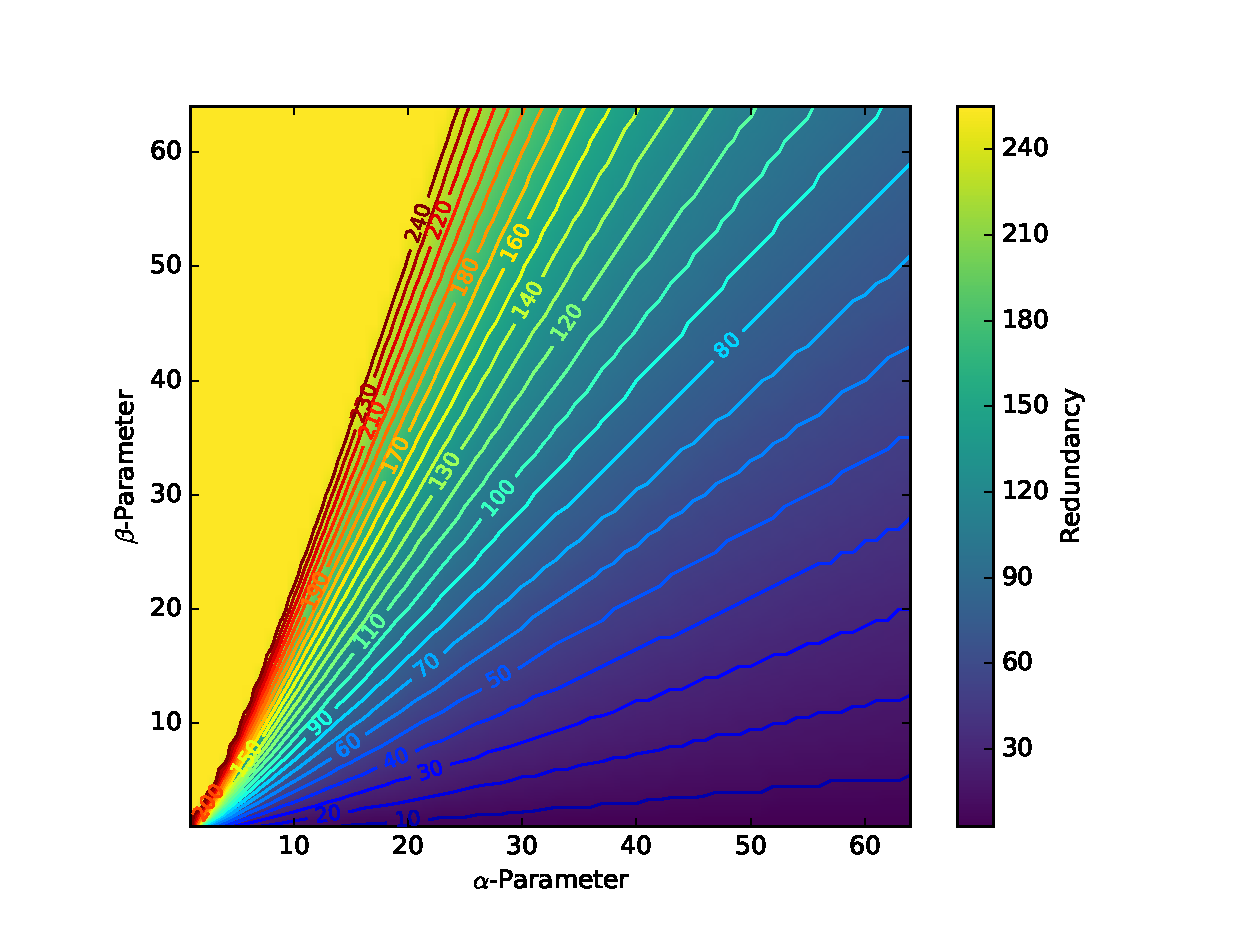
\includegraphics[width=\textwidth]{prediction/cdf-contour}
  \caption{Amount of redundancy required to transmit $64$ packets successfully with a probability of $90\%$ (capped at 250)}
  \label{fig:prediction:cdf-contour}
\end{figure}

\begin{figure}
	\centering
	\begin{subfigure}[b]{0.3\textwidth}
		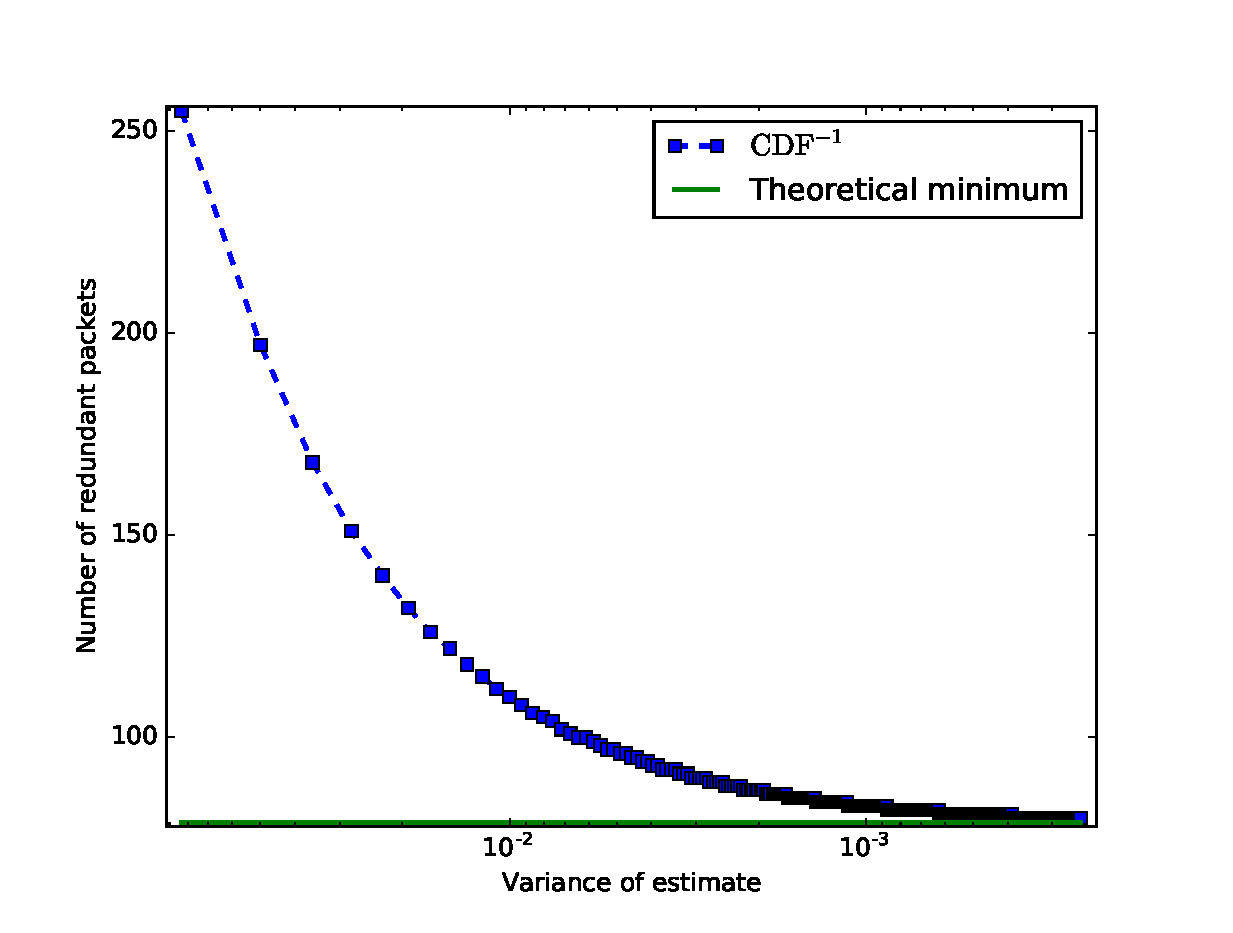
\includegraphics[width=\textwidth]{prediction/converge-0-5}
		\caption{LQ of $50\%$}
	\end{subfigure}
  \begin{subfigure}[b]{0.3\textwidth}
		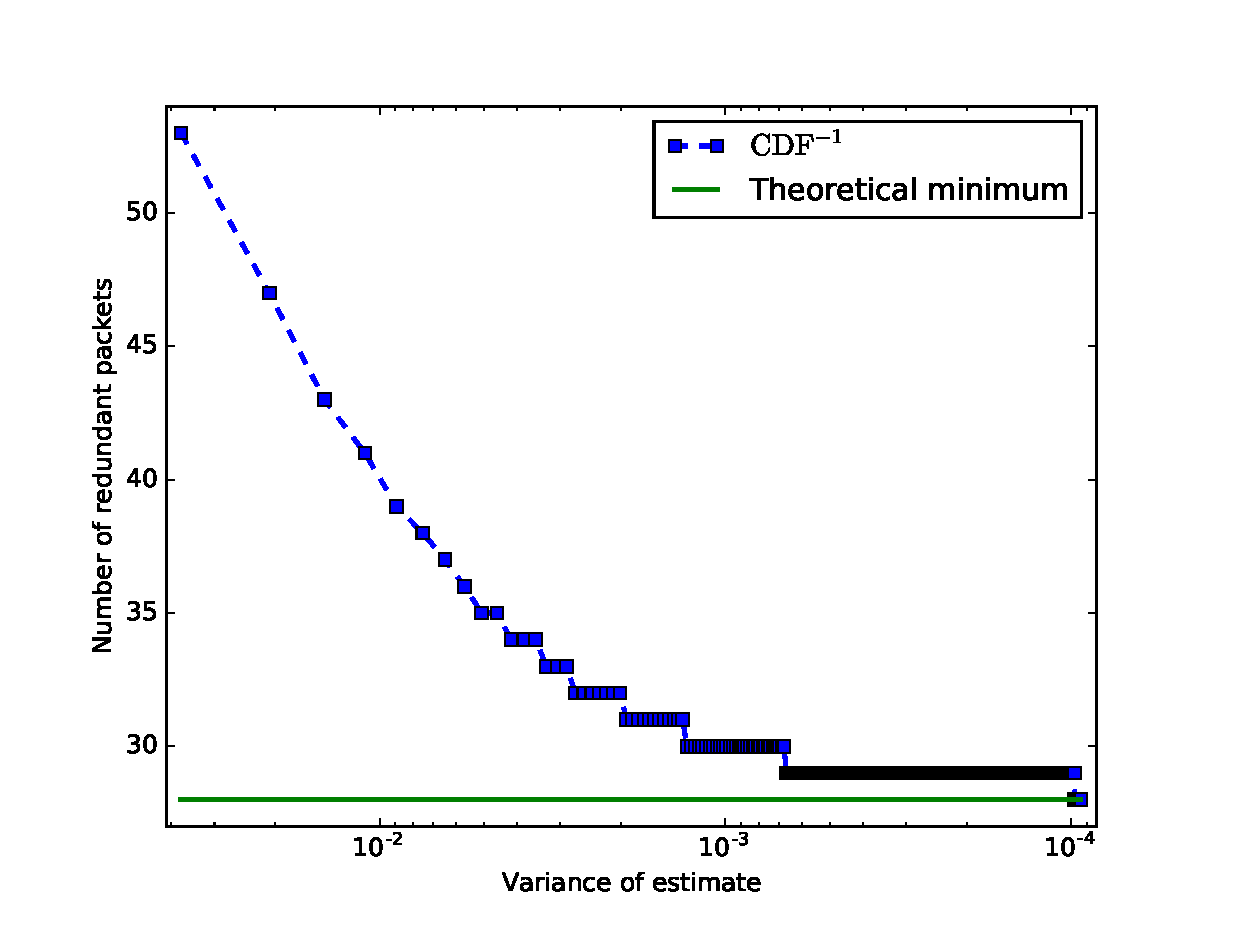
\includegraphics[width=\textwidth]{prediction/converge-0-75}
		\caption{LQ of $75\%$}
	\end{subfigure}
  \begin{subfigure}[b]{0.3\textwidth}
		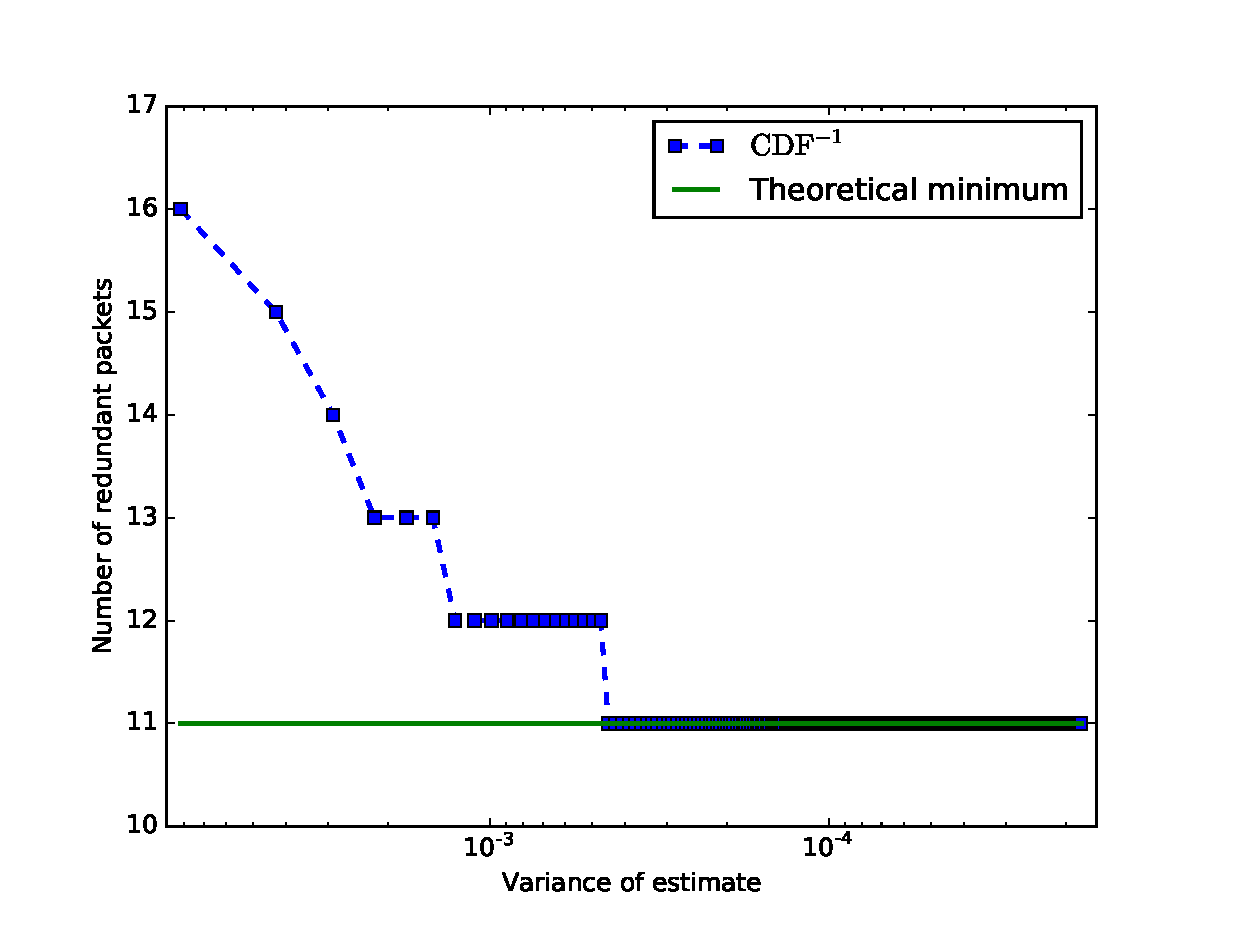
\includegraphics[width=\textwidth]{prediction/converge-0-9}
		\caption{LQ of $90\%$}
	\end{subfigure}
	\caption{Amount of redundancy required to transmit $64$ packets successfully with a probability of $90\%$}
  \label{fig:prediction:convergence}
\end{figure}

\section{Linux}

At least some of linux's wireless drivers use exponential moving average.

\begin{minted}{c}
  static void atmel_smooth_qual(struct atmel_private *priv)
  {
    unsigned long time_diff = (jiffies - priv->last_qual) / HZ;
    while (time_diff--) {
      priv->last_qual += HZ;
      priv->wstats.qual.qual = priv->wstats.qual.qual / 2;
      priv->wstats.qual.qual +=
        priv->beacons_this_sec * priv->beacon_period * (priv->wstats.qual.level + 100) / 4000;
      priv->beacons_this_sec = 0;
    }
    priv->wstats.qual.updated |= IW_QUAL_QUAL_UPDATED;
    priv->wstats.qual.updated &= ~IW_QUAL_QUAL_INVALID;
  }
\end{minted}

\section{Validating the assumptions}
We have run a few experiments that try to justify the modeling decisions earlier. We present the results here.

\subsection{Autocorrelation test}
In Section \ref{sec:model} we modelled subsequent packet transfers as independent actions with dependent probabilities.
If, however, packet transfers were dependent, this could break the assumptions made when using the negative binomial distribution and require higher redundancy.
Unfortunately, it is not directly feasible to test whether random variables are independent.
However, in many situations dependent variables are also correlated. (But not in all. Only the converse is an implication.)
Thus, we ran a series of experiments with one node transmitting at constant rate and another node tracking which packets it received.
We varied the channel ($\SI{5700}{\mega\hertz}$, $\SI{4920}{\mega\hertz}$, $\SI{5240}{\mega\hertz}$), the frame length ($\SI{28}{\byte}$, $\SI{528}{\byte}$, $\SI{1028}{\byte}$), and the injection rate ($\SI{2}{\per\second}$, $\SI{100}{\per\second}$, maximum (depends on MCS index and frame length, $\SI{4500}{\per\second}$, ranged between and $\SI{7000}{\per\second}$)).
Figure \ref{fig:acrpil} shows a few exemplary autocorrelation plots.
These plots were generated on a vector where a 1 indicates a received packet and a 0 a loss.

\begin{figure}
	\centering
	\begin{subfigure}[b]{0.45\textwidth}
		\includegraphics[width=\textwidth]{./fig/maes-1456822952-5240-2-3-modpc.png}
		\caption{MCS 3, 2 frames per second,\\ $\SI{5240}{\mega\hertz}$, $\SI{28}{B}$}\label{fig:acrpil:a}
	\end{subfigure}
	\begin{subfigure}[b]{0.45\textwidth}
		\includegraphics[width=\textwidth]{./fig/maes-1456906587-5700-100--1000pc.png}
		\caption{MCS 3, 100 frames per second,\\ $\SI{5700}{\mega\hertz}$, $\SI{1028}{B}$}\label{fig:acrpil:b}
	\end{subfigure}
	\begin{subfigure}[b]{0.45\textwidth}
		\includegraphics[width=\textwidth]{./fig/maes-1456822952-5240-2-2-modpc.png}
		\caption{MCS 2, 2 frames per second,\\ $\SI{5240}{\mega\hertz}$, $\SI{28}{B}$}\label{fig:acrpil:c}
	\end{subfigure}
	\begin{subfigure}[b]{0.45\textwidth}
		\includegraphics[width=\textwidth]{./fig/maes-1456822952-5240-20000-2-modpc.png}
		\caption{MCS 2, 6052 frames per second,\\ $\SI{5240}{\mega\hertz}$, $\SI{28}{B}$}\label{fig:acrpil:d}
	\end{subfigure}
	\caption{Autocorrelation plots of constant rate packet injection loss}\label{fig:acrpil}
\end{figure}

Subfigures \ref{fig:acrpil:a} and \ref{fig:acrpil:b} show normal behavior of the correlation values remaining between the confidence bounds (plotted as blue lines around 0) and show no indication of changing over time.
Subfigure \ref{fig:acrpil:c} shows a correlation that drags over a long period ($\SI{200}{\second}$ are shown in the plot) and can easily be compensated by learning the new channel properties.
Subfigure \ref{fig:acrpil:d} shows one of the few cases where we discovered a correlation over a short period of time, about $\SI{200}{\milli\second}$ in this case.
However, the correlation is not dramatic and can be safely ignored.

\subsection{A stress test}

One of the hardest problems to deal with in an encoded packet network % Marten: Eigentlich heißen die coded packet network, aber irgendwann brauchten Stephan mal ein Backronym für moep (sein Spitzname). Und da kam mesh over encoded packets auf. Mal gucken, ob er's mitbekommt. :)
is starting up from beacon traffic to transmitting at maximum possible rate.
In such a situation, the reliable transfer of a generation can only be ensured by inserting large amounts of redundancy.
This section asks the question: when applied to such a situation, does our model predict the right amount of redundancy?

We set up the following experiment with two participants, A and B:
A remains at beacon traffic of 5 frames per second for 24 seconds to obtain a somewhat stable estimate of the channel.
These estimates are communicated back by B.
After 24 seconds, A derives the number of frames that has to be sent so that 64 frames or more are received (i.e.\ a generation of 64 packets could be decoded) with a probability of $0.9$ at B.\footnote{The code for this experiment is included in \texttt{experiments/burstsend/} of the accompanying file repository.}

The experiment has been conducted at $\SI{5825}{\mega\hertz}$, HT20, MCS index 10, and a frame length of 28B.
As a trust function (see Section \ref{sec:trust_function}), we used $e^{-\nicefrac{t}{3}}$, where $t$ is the time in seconds.

We repeated this experiment 1012 times.
In 940 cases, 64 or more frames were received, indicating a (generation) success rate of approx.\ $0.94$, slightly above the desired rate of $0.9$.

Closer inspection of the data revealed the following:
the estimator indicated that more than 128 frames would be necessary in 8 cases.
Out of these cases, only 3 succeeded with 64 or more frames received.
An investigation towards the reasons of this is left for future work.
We deem it likely that this happened merely due to the fact that the channel became unstable at the moment of the experiment (in general, the frame success rate was about $0.83$) and no safe prediction could be made.

\subsection{Full load test}
To complement the first, low load experiment, we ran a second one with full load from A to B.
Essentially, the experiment remained the same as in the previous section, only that the waiting time of 24 seconds between the bursts was removed.
Additionally, we had to downgrade the MCS index to 8.
When attempting the experiment with the original MCS index, we saw the packet success probability quickly declining over the first 10 to 20 seconds.\footnote{%
	We speculate that this is due to the hardware warming up, increasing the loss rate.}
We thus reduced the MCS index and removed the values up to a point where the packet success probability stabilized.
Additionally, we increased the rate at which the parameters $\alpha$ and $\beta$ were communicated back by B to match the rate of generations

Out of the 1067 generations sent, B received 64 more frames in 979 cases, indicating a generation success probability of $0.92$.
The packet success rate was at $0.921$.

When preparing for this second test, we noticed that the chosen trust function is too optimistic for a real network setup.
While it produced the expected results in the final setup, a quickly changing packet success probability decreased the generation success probabilities to $0.8$ and lower.
This could already be triggered by a person moving around in the same room, changing the link quality.
Choosing a different trust function, e.g., $e^{-xt}$ $x=1$ might help to solve this.
Finding an appropriate parameter $x$ that works in many situations, especially outside of laboratory conditions, is left for future work.

\subsection{Perfect channel test}
On a channel with perfect link quality and high throughput, eventually 0 redundancy will be inserted.
On a near-perfect channel with packet success probabilities >0.99, a single packet of redundancy remains.

\end{document}
